\documentclass{article}
\usepackage{graphicx}
% numeric citation style: \citet -> "Gurnee et al. [1]", \citep -> "[1]"
\PassOptionsToPackage{numbers, sort&compress}{natbib}

% The authors should use one of these tracks.
% Before accepting by the NeurIPS conference, select one of the options below.
% 0. "default" for submission
%\usepackage{neurips_2026}
% the "default" option is equal to the "main" option, which is used for the Main Track with double-blind reviewing.
% 1. "main" option is used for the Main Track
%  \usepackage[main]{neurips_2026}
% 2. "position" option is used for the Position Paper Track
%  \usepackage[position]{neurips_2026}
% 3. "eandd" option is used for the Evaluations & Datasets Track
 % \usepackage[eandd]{neurips_2026}
% 4. "creativeai" option is used for the Creative AI Track
%  \usepackage[creativeai]{neurips_2026}
% 5. "sglblindworkshop" option is used for the Workshop with single-blind reviewing
\usepackage[dblblindworkshop]{neurips_2026}
% 6. "dblblindworkshop" option is used for the Workshop with double-blind reviewing
%  \usepackage[dblblindworkshop]{neurips_2026}
% 7. "education" option is used for the Education Track
%  \usepackage[education]{neurips_2026}


% After being accepted, the authors should add "final" behind the track to compile a camera-ready version.
% 1. Main Track
 % \usepackage[main, final]{neurips_2026}
% 2. Position Paper Track
%  \usepackage[position, final]{neurips_2026}
% 3. Evaluations & Datasets Track
 % \usepackage[eandd, final]{neurips_2026}
% 4. Creative AI Track
%  \usepackage[creativeai, final]{neurips_2026}
% 5. Workshop with single-blind reviewing
%  \usepackage[sglblindworkshop, final]{neurips_2026}
% 6. Workshop with double-blind reviewing
%  \usepackage[dblblindworkshop, final]{neurips_2026}
% Note. For the workshop paper template, both \title{} and \workshoptitle{} are required, with the former indicating the paper title shown in the title and the latter indicating the workshop title displayed in the footnote.
% For workshops (5., 6.), the authors should add the name of the workshop, "\workshoptitle" command is used to set the workshop title.
\workshoptitle{InterpScience}
% 7. Education Track
% \usepackage[education, final]{neurips_2026}

% "preprint" option is used for arXiv or other preprint submissions
 % \usepackage[preprint]{neurips_2026}

% to avoid loading the natbib package, add option nonatbib:
%    \usepackage[nonatbib]{neurips_2026}
 \usepackage{amsmath}
\usepackage[utf8]{inputenc} % allow utf-8 input
\usepackage[T1]{fontenc}    % use 8-bit T1 fonts
\usepackage{hyperref}       % hyperlinks
\usepackage{url}            % simple URL typesetting
\usepackage{booktabs}       % professional-quality tables
\usepackage{amsfonts}       % blackboard math symbols
\usepackage{nicefrac}       % compact symbols for 1/2, etc.
\usepackage{microtype}      % microtypography
\usepackage{xcolor}         % colors
\usepackage{verbatim}       % provides the comment environment

% shorthand used in the cross-modal math
\newcommand{\img}{\mathrm{img}}
\newcommand{\txt}{\mathrm{txt}}

\newcommand{\clip}{\mathrm{clip}}

% component index and alignment metric, used everywhere
\newcommand{\fl}{\mathrm{full}}
\newcommand{\mnn}{\mathrm{m\text{-}NN}}

% Note. For the workshop paper template, both \title{} and \workshoptitle{} are required, with the former indicating the paper title shown in the title and the latter indicating the workshop title displayed in the footnote. 
\hypersetup{pdftitle={Not All Representational Convergence Is Semantic:
    Measuring Alignment in the Jacobian Subspace}}
\title{Not All Representational Convergence Is Semantic: Measuring Alignment in the Jacobian Subspace}

% The \author macro works with any number of authors. There are two commands
% used to separate the names and addresses of multiple authors: \And and \AND.
%
% Using \And between authors leaves it to LaTeX to determine where to break the
% lines. Using \AND forces a line break at that point. So, if LaTeX puts 3 of 4
% authors names on the first line, and the last on the second line, try using
% \AND instead of \And before the third author name.


\author{%
  Alexander Zhang \\
  University of Oxford
  \And
  Michael Shihong Zhang \\
  University of Waterloo
  % examples of more authors
  % \And
  % Coauthor \\
  % Affiliation \\
  % Address \\
  % \texttt{email} \\
  % \AND
  % Coauthor \\
  % Affiliation \\
  % Address \\
  % \texttt{email} \\
  % \And
  % Coauthor \\
  % Affiliation \\
  % Address \\
  % \texttt{email} \\
  % \And
  % Coauthor \\
  % Affiliation \\
  % Address \\
  % \texttt{email} \\
}
\begin{document}

\maketitle

\begin{abstract}
  The Platonic Representation Hypothesis~\citep{huh2024platonic} asserts that neural networks converge towards a shared representation of reality as they become more competent. Evidence for this has thus far come from the full activation space, where alignment between two models rises with their competence. However, this comparison mixes semantic content with superficial regularities like document length and syntax. We instead measure alignment in the Jacobian space (J-space), the privileged subspace induced by the Jacobian lens (J-lens)~\citep{gurnee2026verbalizable}, and find it is a more semantically selective measure. 
  
  Re-examining convergence by comparing kernels induced by the J-space, we still find that models converge: the Spearman correlation between competence and alignment is $\rho = 0.56$, $p = 0.016$ among language models and $\rho = 0.97$, $p < 10^{-4}$ between language models and vision encoders. Within-language, though, the J-space converges much more slowly than the full activation space, so part of the apparent link between competence and convergence is carried by superficial structure. Consistent with this, the gap between J-space and full convergence disappears across modalities, where no such structure is shared.
  
  This convergence is also legible: using the J-lens at matched layer depth, independently trained models name 5.0 of 25 shared vocabulary items above a position-shuffled floor against 1.9 for the plain logit lens. J-lens overlap converges with competence similarly to the kernel measure, at $\rho = 0.73$, $p=0.0021$. Code available at \url{https://github.com/excelexx/jspace-convergence}.
\end{abstract}
\section{Introduction}
The Platonic Representation Hypothesis~\citep{huh2024platonic} asserts that
``Neural networks, trained with different objectives on different data and
modalities, are converging to a shared statistical model of reality in their
representation spaces.'' Concretely, the claim is that alignment between two models grows with their competence. To our knowledge, alignment has thus far been computed over the full representational spaces\footnote{We say ``full activation space'' rather than the ``full representational space'', since every quantity we compare is a mean-pooled residual-stream vector at a given layer.}. We show this method conflates semantic content with confounding surface-level similarities like syntax, length and formatting. 

Recently, \citet{gurnee2026verbalizable} introduced a new interpretability
technique, the Jacobian lens (J-lens), which recovers the concepts a language model is poised to verbalise at a given layer. The J-lens induces the J-space, a privileged subset of internal representations available for report and reasoning. The subspace is both semantically significant, acting as a ``global workspace'' for the model, and privileged, capturing a median of only 6--7\% of a concept vector's variance~\citep{gurnee2026verbalizable}.

Thus, we hypothesise that the J-space will provide a more semantically selective measure of convergence than the full activation space, in the sense that J-space alignment will drop more sharply when semantic content is removed. 

\paragraph{Motivating experiment}
We compute alignment using ``mutual $\kappa$-nearest-neighbour overlap'' between pairs of models. We do this once on an ordinary dataset of text documents and once on the same documents with content words randomised but sentence structure preserved. We find that over half of the full alignment is retained, compared with a quarter of J-space alignment. After running a random-dictionary control, we find that roughly two thirds of this drop in retention is explained by the sparse coding rather than the J-lens dictionary, but the remaining third is attributable to the J-space. 

We use the J-space to re-examine the Platonic Representation Hypothesis's central claim, and find that models do indeed converge under this stricter measure.

Our three experiments compare 1) J-space against full alignment for text models (including the content-ablated motivating experiment); 2) text models against vision encoders, which have no J-space of their own; and 3) the J-lens readouts of text models, where outputs are vocabulary tokens and no machinery is needed. For each case, we test convergence by relating alignment to competence. The third experiment also compares against the logit lens~\citep{nostalgebraist2020logitlens} to determine whether agreement is attributable to the Jacobian or merely to models predicting similar next words at similar depths.


\paragraph{Related work}
Representational similarity has been measured in many ways: RSA compares dissimilarity matrices~\citep{kriegeskorte2008rsa}, SVCCA compares subspaces through canonical correlation~\citep{raghu2017svcca}, and centred kernel alignment compares item--item kernels, with invariance to orthogonal transformation and isotropic scaling~\citep{kornblith2019cka}. \citet{huh2024platonic} measure convergence using mutual $\kappa$-nearest-neighbour overlap~\citep{bestbuddies} and CKNNA.

Whether these alignment scores place weight onto semantic content, however, is less settled. \citet{ding2021grounding} show that similarity measures can disagree with functional measures of model behaviour, and validations of these measures
have largely focused on whether layers correspond across models, rather than whether such measures isolate meaning. 

To our knowledge, previous work varies the \emph{metric}, while always comparing the full activation space. In contrast, we hold the metric fixed and restrict the comparison to a specific \emph{subspace}. 

Since the J-space is defined by the Jacobian to the output, it discards directions that cannot affect the model's predictions. Therefore, we still compare representations, but unlike previous work, restrict our attention to representations which have functional consequences.

\paragraph{Contributions} 
\begin{enumerate}
\item We propose measuring alignment between models in the J-space rather than the full activation space, and we validate the J-space as a semantically selective measure of alignment using an intervention. We find that randomising content words removes 74\% of J-space alignment but only 46\% of full-activation alignment.
\item We find that part of the existing competence--convergence relationship rests on structure that is shared, but not semantic. Indeed, within language, J-space alignment rises with competence at roughly a third the rate of full activation space, while across modalities the two rates are indistinguishable. 
\item We show that J-space convergence is meaningful and can be read as words using the J-lens. At matched relative layer depth, independently trained models name 5.0 of 25 shared vocabulary words against 1.9 for the plain logit lens. J-lens readouts also converge as competence increases, at least as closely as the kernel measure.
\end{enumerate}

\section{Formal setup}
\label{sec:formal}
We first define the alignment measure used in Experiments 1 and 2. Our third experiment needs no machinery beyond the J-lens itself, since the readouts are in a shared vocabulary space.

For the first two experiments there is no such shared output space. For
instance, two models may have different residual widths or different
modalities. We therefore adapt the method of \citet{huh2024platonic}, which
measures alignment by kernels rather than
the representations themselves. Between language models, we compare the kernels induced by the J-spaces of
the models. Across modalities, we compare the kernel induced by the J-space of
the text model to the kernel built from raw pooled patch features.

Let $A, B,\dots$ denote language models with residual widths $r_A, r_B, \dots$
and layer counts $L_A, L_B, \dots$ that generally differ. We index layers by
$\ell \in \{0,\dots,L_A-1\}$ and write $p = \ell/(L_A-1) \in [0,1]$ for the
corresponding \emph{relative depth}.

We consider alignment over input items. For
text--text comparisons, item $i$ is a document and both models receive it. For text--vision comparisons, item $i$ is an image--caption pair, with the vision encoder receiving the image and the language model receiving the caption. For each model, layer $\ell$, and item $i$, we mean-pool the residual stream over the item's tokens or patches, giving $h^{A,(\ell)}_i \in \mathbb{R}^{r_A}$.

For each language model, we compute the fitted J-lens~\citep{gurnee2026verbalizable}.
\[
  J^A_\ell \;=\;
  \mathbb{E}_{i}\!\left[\;
    \mathbb{E}_{(s' \geq s)}\!
    \left[ \frac{\partial h^{A,(\mathrm{final})}_{s',i}}
      {\partial h^{A,(\ell)}_{s,i}} \right]
    \right]
  \;\in\; \mathbb{R}^{r_A \times r_A},
\]
where $s$ and $s'$ index tokens with $s' \geq s$, since a token cannot affect
its predecessors.

Let $W_U^A \in \mathbb{R}^{m_A \times r_A}$ be model $A$'s unembedding matrix,
mapping its final residual stream to $m_A$ vocabulary logits. We preprocess
$W_U^A$ by folding in the gain $w^A$ of model $A$'s final normalisation layer and centring it over the $m_A$ output coordinates:
\[
  \widetilde{W}_U^A \;=\; \left(I_{m_A} - \frac{1}{m_A}\mathbf{1}\mathbf{1}^{\top}\right) W_U^A \operatorname{diag}(w^A), \qquad \mathbf{1}\in\mathbb{R}^{m_A}
\]
Without centring, the coefficients for the decomposition in the next step can collapse to near-zero.

The J-space dictionary for layer $\ell$ of model $A$, with rows $d^A_{\ell,v}$ that are directions in residual-stream space, is
\[  D^A_\ell \;=\; \widetilde{W}_U^A J^A_\ell \;\in\; \mathbb{R}^{m_A \times r_A}.
\]

\subsection{Decomposing activations into the J-space and remainder}
We decompose each pooled activation into the J-space and non-J remainder, writing each activation as a sparse non-negative combination of $k=25$ J-space dictionary directions. For tractability, we use a greedy orthogonal matching pursuit (OMP) to select a subset $\mathcal{S}_i$ of dictionary coordinates with $|\mathcal{S}_i|=k$. We then refit the coefficients $\alpha_{i,v}$, where $v \in \mathcal{S}_i$, with a projected-gradient non-negative least-squares (NNLS) step. 

Denote the normalised unit directions as $\bar{d}^A_{\ell,v}$ and $h^{A,(\ell)}_{\fl,i} \equiv h^{A,(\ell)}_i$ as the full pooled activation. Then, we have
\[
  h^{A,(\ell)}_{J,i} = \sum_{v \in \mathcal{S}_i} \alpha_{i,v}\, \bar{d}^A_{\ell,v},
  \qquad
  h^{A,(\ell)}_{\perp,i} = h^{A,(\ell)}_{\fl,i} - h^{A,(\ell)}_{J,i}
\]

We thus consider three components, written $h^{A,(\ell)}_{\omega,i}$ for
$\omega \in \{\fl, J, \perp\}$: the full activation $h^{A,(\ell)}_{\fl,i}$, the
J-space component $h^{A,(\ell)}_{J,i}$, and the non-J remainder
$h^{A,(\ell)}_{\perp,i}$. Our aim is to compare alignment computed from each.

\subsection{Kernels}
Each component is winsorised at the 95th percentile and normalised to unit magnitude, and we denote the preprocessed components by $\hat{h}^{A,(\ell)}_{\omega,i}$. The kernel for model $A$, layer $\ell$, and component $\omega$ is the $n \times n$ matrix of cosine similarities between items, 
\[
  K^{A,\omega}_{\ell}(i,j)
  =
  \left \langle \hat{h}^{A,(\ell)}_{\omega,i},\, \hat{h}^{A,(\ell)}_{\omega,j} \right\rangle.
\]

The dictionaries of text models have one row per vocabulary token, making the induced kernels
interpretable~\citep{geva2022transformer,dar2023analyzing}. However, vision
encoders have no such equivalent: MAE~\citep{he2021maskedautoencodersscalablevision} decodes to raw pixels, and DINOv2~\citep{oquab2024dinov2learningrobustvisual} 
decodes to abstract prototypes. We thus only apply the J-lens to the caption side, building image kernels from
raw pooled patch features, so on the image side, only $\omega = \fl$ is defined. The image kernel $K^{\img,\,\fl}_{\ell}$ is formed by the same cosine-similarity expression from the preprocessed\footnote{The image side is winsorised per coordinate at the $0.5$th and $99.5$th percentiles, then normalised to unit magnitude.} mean-pooled patch activations.

\subsection{Mutual \texorpdfstring{$\kappa$}{kappa}-nearest-neighbour alignment}
We compare two kernels through mutual $\kappa$-nearest-neighbour overlap~\citep{bestbuddies}. Taking each item's $\kappa$ nearest neighbours under each kernel (the $\kappa$ largest off-diagonal entries of its row), we define $\mnn(K^{A,\omega}_{\ell},\, K^{B,\omega'}_{\ell'})$ between layer $\ell$ of model $A$ and layer $\ell'$ of model $B$ as the average fraction of overlapping neighbours shared by the two kernels, over all $n$ items.

For a text--text comparison both sides carry the same component, $\omega' =
  \omega$. For a text-to-vision comparison the caption side varies over $\omega
  \in \{\fl, J, \perp\}$ while the image side is fixed at $\omega' = \fl$.

Finally, we define the alignment between $A$ and $B$ for component $\omega$ as
the mean over layer pairs $(\ell, \ell') \in \mathcal{B}_A \times \mathcal{B}_B$, where
$\mathcal{B}_A = \{\,\ell : 0.35 \le \ell/(L_A-1) \le 0.90\,\}$ is the relative layer depth band:

\[
  \mathcal{A}^{\omega}(A,B) \;=\; \operatorname{mean}_{\ell, \ell'}\mnn\big(K^{A,\omega}_{\ell},\, K^{B,\omega'}_{\ell'}\big)
\]

\section{Experiment setup}
\subsection{Text--text alignment and motivating experiment}
We compare the following 11 text models of varying size and
architecture: Pythia-70M~\citep{biderman2023pythia}, GPT-2~\citep{radford2019language}, Gemma-3-270M~\citep{gemmateam2025gemma3technicalreport}, Qwen3.5-0.8B~\citep{qwen35blog}, Gemma-3-1B,
Qwen3-1.7B~\citep{qwen3}, Qwen3.5-2B, Gemma-2-2B~\citep{gemmateam2024gemma2improvingopen}, Qwen3-4B, Qwen3.5-4B, Gemma-3-4B~\citep{gemmateam2025gemma3technicalreport}.

For the first experiment, we use the prefitted J-lenses on Neuronpedia~\citep{neuronpedia}, and compute alignment across all $\binom{11}{2}=55$
text--text pairs on 1,000 documents from pile-10k~\citep{Nanda2022Pile10K},
a subset of the Pile~\citep{gao2020pile800gbdatasetdiverse}, following
Section~\ref{sec:formal}. We take the first 1,000 rows, truncate each to at
most 1,500 characters, then to at most 300 tokens, and mean-pool over token
positions. Any difference in tokeniser efficiency is quite marginal, from
$3.79$ to $4.19$ characters per token. Measured over the corpus, the least efficient tokeniser still ingests 94.8\% as many characters per document as the most efficient. Neighbourhoods are taken at $\kappa=10$.

Following the procedure described in the previous section, we evaluate shared
semantic content for the J-space, the non-J remainder, and the full activation space
over the original corpus. We then repeat the measurement on a content-ablated
variant of the same 1,000 documents. We preserve syntactic structure, replacing each non-stopword alphabetic token (i.e. content words) with another drawn from the same log-frequency bin. For example,
``Remember that children each progress at their own rate.'' becomes ``Reduce that
self each rates at their own special.''
Comparing these two results isolates how much of each component's alignment is
semantic.

We then conduct a random-dictionary control to assess how much of the
retention drop comes from the sparse coding of the J-space: we run a Gaussian
dictionary through the same content-ablation test and report its retention rate.

Finally, we relate alignment to competence, measuring\footnote{All benchmark results were self-computed to ensure consistency.} model competence with the HellaSwag
benchmark~\citep{zellers2019hellaswagmachinereallyfinish}. Appendix~\ref{app:competence} repeats the analysis with different competence axes.

\subsection{Text-vision alignment}
For our second experiment, we compare DINOv2, MAE, CLIP~\citep{radford2021learningtransferablevisualmodels}, and SigLIP~\citep{zhai2023sigmoidlosslanguageimage} against the 11 language models for a total of $4 \times 11 = 44$ text--vision model pairs. All four are ViT-Base encoders~\citep{dosovitskiy2021imageworth16x16words} with different pretraining objectives. Alignment is computed as in Section~\ref{sec:formal} over 1,024 image--caption pairs from the Wikipedia-based Image Text (WIT) dataset~\citep{wit}. 

For tractability, we compute mean alignment over a subset of the layers. On the text side, we consider at most\footnote{The layer band for Pythia-70M contains only 2 layers. All other text models use five layers.} five evenly spaced layers from the band $\mathcal{B}_A$. On the vision side, we consider the final hidden state along with five evenly spaced blocks from index $2$ to $\mathrm{final}-2$. For a model pair, this gives $5 \times 6 = 30$ layer pairs.

We consider a competence axis only on the text side, using the same HellaSwag benchmark.

\subsection{Text--text shared J-lens output}
For our third experiment, we apply the prefitted J-lenses per model and per layer over 200 documents in the
pile-10k dataset~\citep{Nanda2022Pile10K}. Each document is first truncated to 1,500 characters, then to at most 300 tokens. We read the lens out as words, keeping the top $t=25$ entries.
\[
  \mathrm{lens}^A_\ell(h) \;=\; \mathrm{softmax}\!\left(W_U^A\,
  \mathrm{norm}^A\!\left(J^A_\ell h\right)\right).
\]
Since the 11 models do not share a tokeniser, we restrict the J-lens to the 31,548 single-token strings in all 11 vocabularies. We also index positions by character rather than by token, evaluating at 6,000 character positions that fall at a token-end word boundary in all 11 tokenisers.

We then measure how many of the $t=25$ words are shared between model pairs as a function of relative layer depth $p = \ell/(L_A-1)$. We report this overlap minus the readout overlap obtained when positions are randomly re-paired. To control for the possibility that the two models are simply predicting similar next
words, we compare against the logit lens~\citep{nostalgebraist2020logitlens}, which reveals what the model would predict if it stopped at a given layer by reading the residual stream directly:
$\mathrm{softmax}(W_U^A\,\mathrm{norm}^A(h))$. As in the first experiment, we then relate the resulting overlap to the mean HellaSwag accuracy of the pair to re-evaluate the convergence trend.

All experiments were run on a single RTX 3080 (10 GB) GPU, taking a total of around 40 hours.
\section{Results}
\begin{table}
  \centering
  \small
  \caption{Alignment on real versus content-ablated documents over 55 model pairs. Retention is the percentage of alignment which survives ablation, and is substantially lower for J-space than for full. The lower block repeats the ablation with the J-lens dictionary replaced by a Gaussian dictionary. Bracketed intervals are 95\% percentile bootstrap confidence intervals over the 55 model pairs (2,000 resamples).}
  \label{tab:surrogate}
  \begin{tabular}{lccc}
    \toprule
             & Real alignment  & Content-ablated alignment  & Retention                                 \\
    \midrule
    \multicolumn{4}{l}{\emph{Components, J-lens dictionary}}                                                   \\
    full     & 0.5577\,{\tiny[0.539, 0.579]} & 0.3009\,{\tiny[0.290, 0.312]} & 54.1\%\,{\tiny[53.01, 55.14]} \\
    non-J     & 0.5057\,{\tiny[0.484, 0.529]} & 0.2609\,{\tiny[0.252, 0.271]} & 52.0\%\,{\tiny[50.73, 53.30]} \\
    J        & 0.4202\,{\tiny[0.409, 0.432]} & 0.1099\,{\tiny[0.108, 0.112]} & \textbf{26.3\%}\,{\tiny[25.63, 27.02]} \\
    \midrule
    \multicolumn{4}{l}{\emph{J-space under a substituted dictionary}}                                          \\
    Gaussian & 0.2103\,{\tiny[0.202, 0.220]} & 0.0719\,{\tiny[0.071, 0.073]} & 34.7\%\,{\tiny[33.66, 35.85]} \\
    \bottomrule
  \end{tabular}
\end{table}
\subsection{Text--text alignment and motivating experiment}
\label{sec:textresults}
When we randomise all content words, the full alignment retains a mean of 54.1\% of its original value, while J-space alignment retains only 26.3\%\footnote{Retention is the mean of per-pair ratios rather than the ratio of means.}. J-space alignment therefore depends more heavily on content than the full activation space.

To test how much of this drop comes from the sparse coding itself, we repeat the ablation experiment with a randomised Gaussian dictionary instead of the J-space dictionary. Under this control, retention is 34.7\%, meaning sparse coding accounts for 69.7\% of the drop between full and J-space retention. However, the remaining third is still attributable to the J-space itself. 

Mean alignment for the J-space ($0.420$), the remainder ($0.506$), and the full activation ($0.558$) is between $42.0\times$ and $55.7\times$ chance level.

Comparing alignment between two models and the mean of their competences, we find a positive correlation across the J-space (Spearman correlation $\rho = 0.56$, $p = 0.016$), full activation ($\rho = 0.77$, $p = 0.0008$), and remainder ($\rho = 0.87$, $p < 0.0001$) over the 55 pairs (Figure~\ref{fig:lobf-components}(a)). Each model appears in ten pairs, so the pairs are not independent; $p$-values thus come from permuting competence across models while holding alignment values fixed.

\begin{figure}[t]
  \centering
  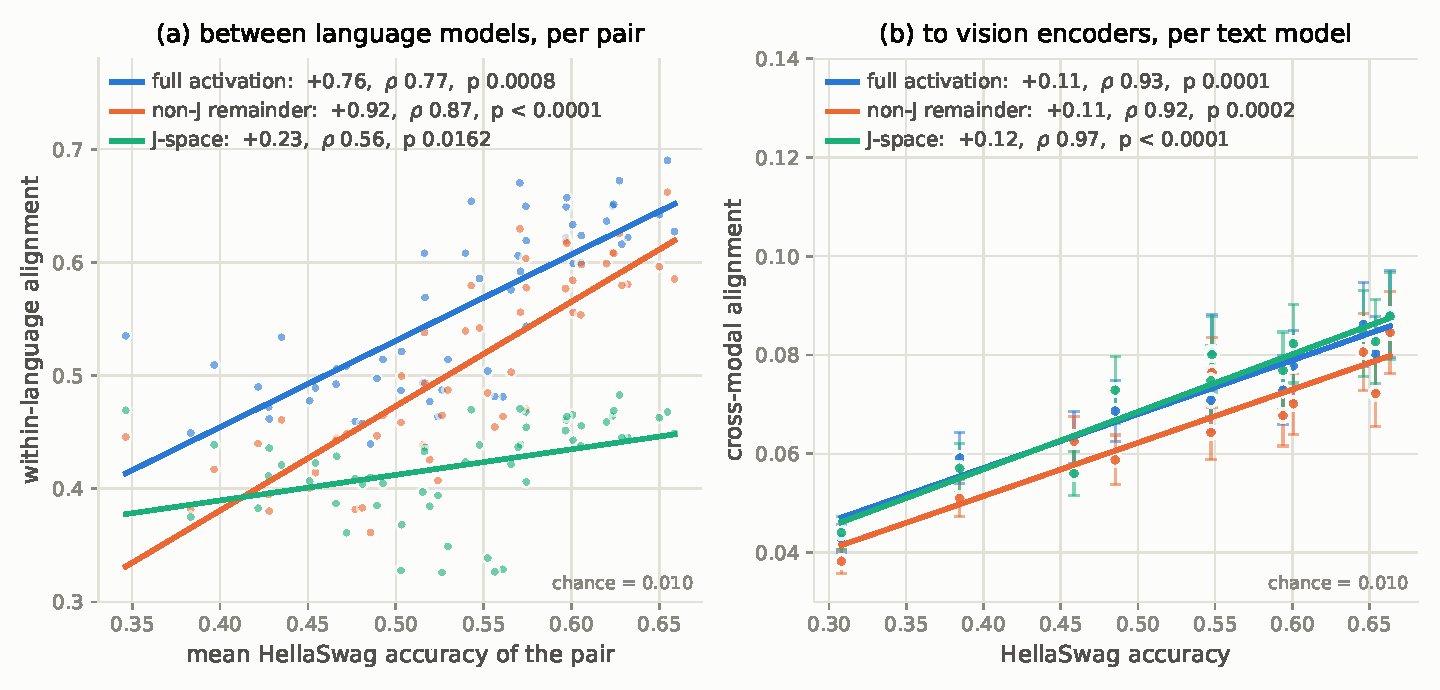
\includegraphics[width=\linewidth]{07_lobf_components.pdf}
  \caption{Alignment graphed against HellaSwag accuracy for full activation, J-space, and non-J remainder, with a line-of-best-fit. \textbf{(a)} Text--text alignment against competence; $p$-values are model-label permutation values. The J-space converges much more slowly than the full activation space. \textbf{(b)} Alignment averaged over the four vision encoders; error bars show standard error of this mean across the four encoders. Alignment
    rises with competence for every component in both settings.}
  \label{fig:lobf-components}
\end{figure}

The rate of convergence in the J-space is about a third of that in the full activation space. Alignment rises with pair competence at $+0.76 \pm 0.09$ per unit HellaSwag accuracy in the full activation space against $+0.23 \pm 0.07$ in the J-space.

\subsection{Comparing text models and vision encoders}

Alignment between text models and vision encoders for each component is between $6.8\times$ and $7.4\times$ chance. Alignment correlates strongly and
positively with competence across the J-space ($\rho = 0.97$, $p< 10^{-4}$), the full activation space ($\rho = 0.93$, $p= 0.0001$), and the remainder ($\rho = 0.92$, $p= 0.0002$). We find that the J-space and full activation converge at nearly identical rates. 

Unlike the text--text comparison, we do not correlate competence with alignment across all 44 text--vision pairs---since the four encoders differ from one another far more than the text models do, this would obscure the actual trend. Indeed, mean J-space alignment ranges from $0.053$ for MAE to $0.087$ for SigLIP, a spread far exceeding the standard deviation of cross-modal alignment across the 11 text models ($0.0134$). 

We instead average alignment within each encoder, then average these four values. We report the four within-encoder correlations, which range from $+0.95$ to $+0.97$, in Appendix~\ref{app:aggregation}.

Cross-modally, there is no shared superficial structure for a full-space metric to capture, so intuitively, J-space and full alignment should match, and they do. Considered alongside Section~\ref{sec:textresults}, where they diverge, this is further evidence that the within-language gap is explained by superficial structure rather than by a property of the J-space.
\subsection{Comparing J-lens shared vocabulary for text models}
\label{sec:wordalign}
We find that at matched relative layer depth, about 5.1 of 25 words are
shared, against 2.0 of 25 for the plain logit lens. Subtracting off the
position-shuffled control, which sits at 0.1 of 25 for the J-lens, we obtain 5.0 of 25
against 1.9 of 25. 

We also find that across the 38
cross-family model pairs, a model's best-matching counterpart layer sits about
11.0\% of the total number of layers away, consistent with Figure~\ref{fig:wordalign-mean-heatmap}. Conducting the same experiment for the logit lens, we find that the J-lens overlap beats the logit-lens overlap in 50/55 pairs, with a median difference of $+11.7\%$ overlap, or $+2.9$ of 25 words. In particular,
in the middle layers $p \in [0.2,0.5]$, J-lens alignment beats logit-lens alignment by 3--5$\times$. The logit-lens comparison rules out the trivial explanation that J-lens alignment is the result of models agreeing on superficial next-token predictions, providing further evidence that the alignment reflects semantically
meaningful content.

\begin{figure}[t]
  \centering
  \begin{minipage}{0.485\linewidth}
    \centering
    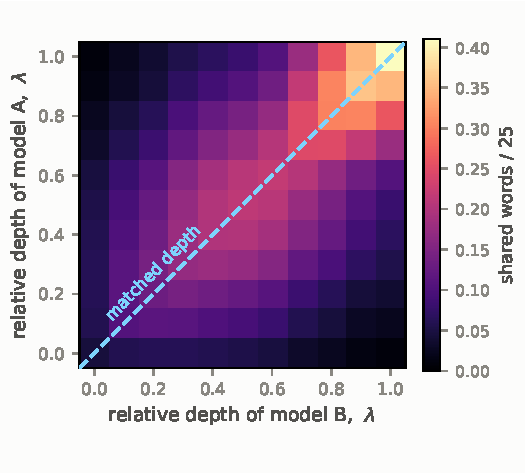
\includegraphics[width=\linewidth]{06_wordalign_mean_heatmap.pdf}\\[2pt]
    \textbf{(a)}
  \end{minipage}\hfill
  \begin{minipage}{0.505\linewidth}
    \centering
    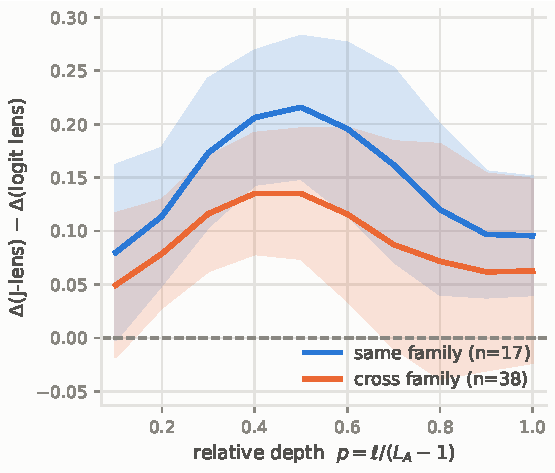
\includegraphics[width=\linewidth]{08_j_minus_logit_vs_depth.pdf}\\[2pt]
    \textbf{(b)}
  \end{minipage}
  \caption{\textbf{(a)} Mean J-lens top-25 word agreement between language models as a
    function of each model's relative layer depth $p = \ell/(L_A-1)$. $\Delta$ is the matched overlap minus the position-shuffled
    overlap; grids are symmetrised before averaging. \textbf{(b)} The shuffle-corrected difference of the J-lens and logit-lens overlap, compared to relative layer depth. $p=0$ is omitted as the logit lens reads the embedding matrix directly, so dominates by construction. Lines are graphed for same-family pairs and cross-family pairs. The shaded region is $\pm 1$ standard deviation across the model pairs in each family group. The mean delta is positive at every depth shown, and peaks in the middle layers. Same-family pairs have noticeably more agreement than cross-family pairs.}
  \label{fig:wordalign-mean-heatmap}
\end{figure}

We also find that J-lens overlap rises with competence, further validating the results of Section~\ref{sec:textresults}. Over the same 55 pairs, $\rho = +0.73$ ($p = 0.0021$), shown in Figure~\ref{fig:wordalign-pairs}. The plain logit lens gives
$\rho = +0.44$, which does not reach significance ($p = 0.085$). 

This readable form of alignment correlates with competence at least as closely as the kernel form, providing further evidence to confirm our claim of convergence.

\begin{figure}[t]
  \centering
  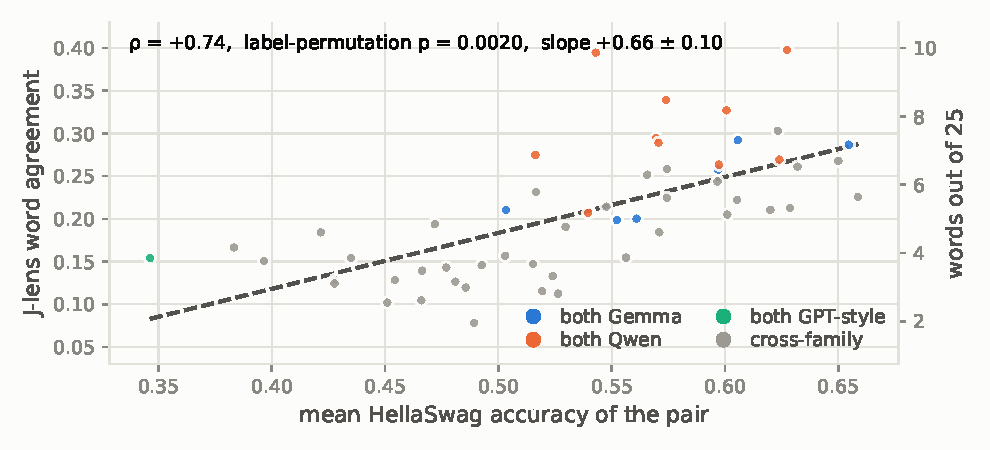
\includegraphics[width=\linewidth]{09_wordalign_pairs_vs_competence.pdf}
  \caption{J-lens top-25 word agreement per model pair against the pair's mean HellaSwag accuracy, coloured by family composition. Each point is the pair's median $\Delta$ (matched overlap minus
    position-shuffled overlap) over the eleven relative layer depths. $p$ is a model-label
    permutation value. Agreement rises with competence.}
  \label{fig:wordalign-pairs}
\end{figure}

\subsection{Controls}
In addition to the random-dictionary control above, we run four further controls:

\paragraph{Random-unembedding-row null}
When we replace the J-lens dictionary with random unembedding rows, J-space alignment exceeds the strongest of five seeded draws in all 55 pairs (mean margin $+0.148$). J-space alignment thus carries information that arbitrary directions do not. For tractability, each null dictionary is a random subset of $20{,}000$ unembedding rows rather than the full dictionary. 

\paragraph{Lens-fitting corpus}
To rule out the possibility that J-space alignment emerges from the shared fitting corpus, we refit so that no two compared models share one. The effect is immaterial (Appendix~\ref{app:lensfit}).

\paragraph{Shuffling image--caption pairs}
Shuffling image--caption pairings in the text--vision alignment experiments reduces alignment to an average of $0.0096$, against a chance level of $0.0098$. Since shuffled pairs share no image--caption relationships, the alignment we measure on the actual pairings is not simply a result of the metric.

\paragraph{Lens degradation}
The J-lens is fitted on ordinary text, so the reduced alignment on the content-ablated documents in the first experiment may be a result of the J-lens simply working less well on such documents. We find that degrading the lens cannot reproduce the effect of removing semantic meaning (Appendix~\ref{app:lensdegrade}).
\section{Conclusion and limitations}

In conclusion, our results suggest that full-space convergence is inflated by surface-level agreement. Within language (where models share superficial regularities), restricting the comparison to the J-space slows convergence to a third of the rate. Across modalities, where no such regularities exist, the two components converge at rates indistinguishable within standard error. Nevertheless, the original convergence claimed by the Platonic Representation Hypothesis still stands, as the J-spaces and J-lenses still align more at higher competence.

This alignment is meaningful and can be read out as actual words. At the same relative layer depth, language models' J-lenses have significant overlap, and this overlap is greater than with the plain logit lens. Measuring convergence with the J-lens reproduces the result of the first experiment, finding that more competent models share a greater J-lens overlap.

\paragraph{Limitations}
First, we test only 11 text models and 4 vision encoders. The text models span 70M--4.3B parameters, and all four vision encoders
are ViT-Base, so we have no competence axis on the vision side. Future experiments on larger models would require fitting of new J-lenses, which is computationally intensive. Furthermore, HellaSwag is near its floor for our smallest models: Pythia-70M scores 30.8\% and GPT-2 scores 38.5\% against 25\% chance. Thus, competence differences at the bottom of the range are highly compressed.

Second, we show the semantic weight of the J-space through only a single method, the retention statistic, and the single randomised dictionary control.

Third, our cross-modal measurement is asymmetric, as for a given image-caption pair, we compare the J-space of a text model to the raw visual representation of the vision encoder.

Fourth, the J-space is a small part of the full activation space, accounting
for an average of 18.3\% of the pooled activation's squared norm across the 11
models. The non-J remainder therefore carries the other 81.7\% of the squared
norm. Our results concern a
minority component of the full activation space, albeit a privileged one, and the
remainder is close enough to the full activation that the two behave nearly
identically.

Fifth, we only test the mutual $\kappa$-NN measure of kernel alignment. Other methods, such as CKA, SVCCA, and CKNNA, may produce different results.

Finally, the J-lens is fitted per token position, but we apply it to mean-pooled document vectors. This means we are assuming that the dictionary's validity transfers to those vectors.
\paragraph{Next steps}
We would like to strengthen our key claim about the J-space's semantic weight with more tests on larger and more varied model types.

We believe that by leveraging the semantically selective properties of the
J-space, we can re-examine many other questions in mechanistic interpretability.
We would also welcome a theoretical account of why the J-space should
be more semantically selective.

Finally, our third experiment compares word overlap rather than activation geometry, which is more functional than representational. Since this paper mostly compares representations, we would welcome future research that uses the J-space to measure functional convergence.

\newpage
\small
\bibliographystyle{plainnat}
\bibliography{references}
\normalsize

%%%%%%%%%%%%%%%%%%%%%%%%%%%%%%%%%%%%%%%%%%%%%%%%%%%%%%%%%%%%

\appendix

\section{Aggregation robustness}
\label{app:aggregation}

Table~\ref{tab:perencoder} gives the cross-modal correlation separately for
each vision encoder. Each encoder has a different alignment level, which is why we consider correlations within encoders rather than pool across all 44 pairs. The relationship holds within every encoder, including MAE,
which receives no text supervision at all. 

\begin{table}[h]
  \centering
  \small
  \caption{Cross-modal alignment against HellaSwag accuracy, computed separately within each vision encoder over the 11 text models. The ``mean J'' column shows alignment for a given encoder across the 11 text models, showing the differences between the encoders that make pooling the 44 pairs inadvisable. $p$-values are exact permutation values for $n=11$.}
  \label{tab:perencoder}
  \begin{tabular}{lcccc}
    \toprule
             & mean J & full                                 & non-J                                 & J                                    \\
    \midrule
    DINOv2  & 0.0742 & $\rho = +0.93$\,{\tiny$p = 0.0001$} & $\rho = +0.92$\,{\tiny$p = 0.0002$} & $\rho = +0.97$\,{\tiny$p < 0.0001$} \\
    MAE     & 0.0535 & $\rho = +0.91$\,{\tiny$p = 0.0003$} & $\rho = +0.92$\,{\tiny$p = 0.0002$} & $\rho = +0.95$\,{\tiny$p < 0.0001$} \\
    CLIP    & 0.0764 & $\rho = +0.93$\,{\tiny$p = 0.0001$} & $\rho = +0.92$\,{\tiny$p = 0.0002$} & $\rho = +0.97$\,{\tiny$p < 0.0001$} \\
    SigLIP  & 0.0865 & $\rho = +0.93$\,{\tiny$p = 0.0001$} & $\rho = +0.92$\,{\tiny$p = 0.0002$} & $\rho = +0.97$\,{\tiny$p < 0.0001$} \\
    \bottomrule
  \end{tabular}
\end{table}

\section{Competence axes}
\label{app:competence}

The main paper measures competence with HellaSwag exclusively. Keeping previous alignment values, we vary the competence scale and derive similar results, shown in Table~\ref{tab:competence} and Table~\ref{tab:crossaxes}.

\begin{table}[h]
  \centering
  \small
  \caption{Spearman rank correlation between within-language alignment and
    competence, per component. The unit is the model pair ($n=55$) and a pair's
    competence is the mean of its two models'. Because each model appears in ten
    pairs the pairs are not independent and a standard $p$-value is invalid; the
    values shown are model-label permutation $p$-values, which hold the
    alignment values fixed and permute competence across models. The alignment
    values are those of Table~\ref{tab:surrogate}; only the competence axis
    varies, here log parameter count and HellaSwag.}
  \label{tab:competence}
  \begin{tabular}{lcc}
    \toprule
         & log parameters ($n=55$)              & HellaSwag ($n=55$)                   \\
    \midrule
    full & $\rho = +0.79$\,{\tiny$p = 0.0006$} & $\rho = +0.77$\,{\tiny$p = 0.0008$} \\
    non-J & $\rho = +0.87$\,{\tiny$p = 0.0002$} & $\rho = +0.87$\,{\tiny$p < 0.0001$} \\
    J    & $\rho = +0.60$\,{\tiny$p = 0.0094$} & $\rho = +0.56$\,{\tiny$p = 0.0162$} \\
    \bottomrule
  \end{tabular}
\end{table}

Table~\ref{tab:crossaxes} repeats the cross-modal comparison of
Figure~\ref{fig:lobf-components}(b) against all three competence measures. We
also measured competence using language-modelling performance, computed as
$1 - \mathrm{bits\text{-}per\text{-}byte}$ over 4M tokens of
OpenWebText~\citep{openwebtext}. We derive similarly strong results across benchmarks as in the main paper.

We follow \citet{huh2024platonic} in using this measure for the cross-modal comparison only, but for the record, this measure gives a within-language J-space correlation of $\rho = +0.35$ ($p = 0.185$), which is not significant.

\begin{table}[h]
  \centering
  \small
  \caption{Spearman rank correlation between cross-modal alignment and
    competence, per component. Each of the 11 text models contributes one point,
    its alignment averaged over the four vision encoders and each layer-pair
    grid reduced by its mean; $p$-values are exact permutation values for
    $n=11$. As in Table~\ref{tab:competence},
    only the competence axis varies, here log parameter count, HellaSwag, and
    $1-$bits-per-byte.}
  \label{tab:crossaxes}
  \begin{tabular}{lccc}
    \toprule
         & log parameters                       & HellaSwag                            & $1-$bits-per-byte                    \\
    \midrule
    full & $\rho = +0.84$\,{\tiny$p = 0.0018$} & $\rho = +0.93$\,{\tiny$p = 0.0001$} & $\rho = +0.96$\,{\tiny$p < 0.0001$} \\
    non-J & $\rho = +0.83$\,{\tiny$p = 0.0022$} & $\rho = +0.92$\,{\tiny$p = 0.0002$} & $\rho = +0.98$\,{\tiny$p < 0.0001$} \\
    J    & $\rho = +0.89$\,{\tiny$p = 0.0005$} & $\rho = +0.97$\,{\tiny$p < 0.0001$} & $\rho = +0.94$\,{\tiny$p < 0.0001$} \\
    \bottomrule
  \end{tabular}
\end{table}
\section{Lens robustness controls}
\subsection{Lens-fitting control}
\label{app:lensfit}
In the main experiment, J-lenses were all fit on the same corpus. As a result, J-space alignment might be a result of the fact that the lenses were fitted on shared text. Figure~\ref{fig:lensfit} recomputes text--text alignment, splitting the fitting corpus into two halves and ensuring the J-lenses of two models in a pair do not use the same half. We also repeat the experiment where two models in a pair share the same half of the fitting corpus. Due to computational constraints, we conduct the control on only 10 pairs (spanning four families) among five models: Pythia-70M, GPT-2, Gemma-3-270M, Qwen3.5-0.8B, and Gemma-3-1B.

We find that corpus-sharing has no measurable impact on alignment. Per-pair differences between the
shared-half and crossed-half conditions have a median of $+0.0002$. All three alignment conditions remain far above the random-dictionary null for every pair.

\begin{figure}[h]
  \centering
  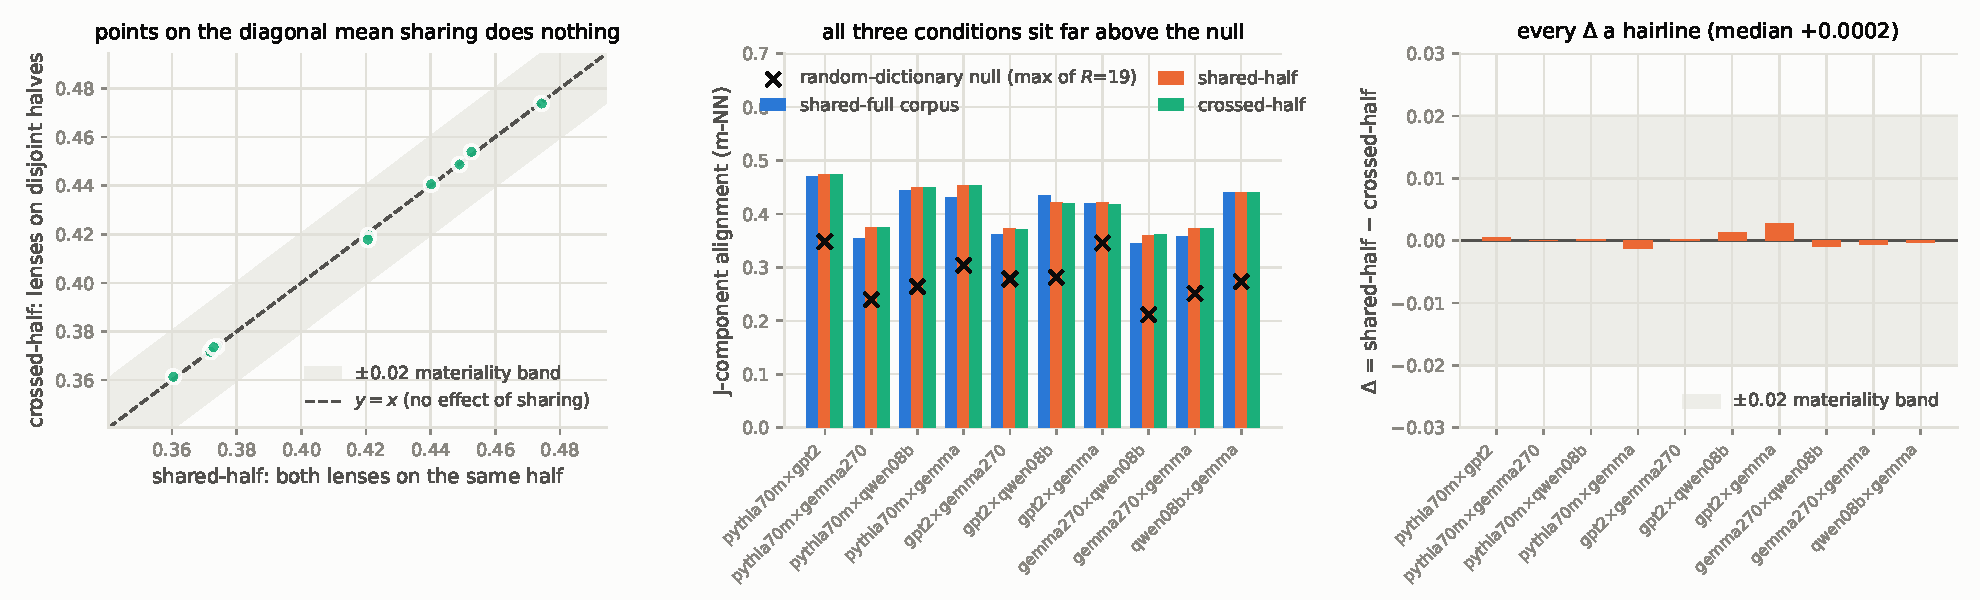
\includegraphics[width=\linewidth]{10_lens_fitting_control.pdf}
  \caption{Disjoint lens-fitting control over the 10 pairs among 5 models. Lenses are fitted on
    disjoint halves of WikiText-103. \textbf{Left:} crossed-half against
    shared-half J-component alignment; points lie on $y=x$ within the $\pm0.02$
    materiality band fixed in advance, so refitting on disjoint halves changes
    nothing. \textbf{Middle:} the three fitting conditions per pair ---
    shared-full corpus, shared-half and crossed-half --- all sit far above the
    per-pair random-dictionary null. \textbf{Right:} the per-pair difference
    $\Delta$ between shared-half and crossed-half, median $+0.0002$ against an
    alignment level of $0.42$, every value inside the band.}
  \label{fig:lensfit}
\end{figure}
\subsection{Lens-degradation control} \label{app:lensdegrade}
The J-lens was fitted only on ordinary text, not content-ablated text, so the reduced alignment on the content-ablated documents may be a result of the J-lens simply working less well on such documents. Indeed, the J-space component accounts for 13.5\% of activations on content-ablated text against 18.3\% on real text. 

We construct an instrument-only null by reducing the number of dictionary directions on the original corpus until the J-space component accounts for the same fraction of the activations as it does on content-ablated text. This gives a J-space that is degraded but computed on documents with intact meaning. Alignment between model pairs with the degraded J-space is $0.2924$ against $0.1099$ for the content-ablated text. Even a
five-direction J-space, which accounts for less of the activation than the 25-direction J-space on content-ablated text, gives alignment $2.1\times$
higher ($0.2326$ against $0.1099$). 

Thus, the lens degradation cannot reproduce the effect of removing semantic meaning.
\newpage
\input{checklist.tex}

\end{document}